\section{Metaheurística de Grasp}

\subsection{Algoritmo}

\indent Nuestra implementación de Grasp opera de la siguiente manera: Se generan una cantidad de veces determinada por parámetro de soluciones con nuestra implementación de la heurística golosa. Luego se elige una de ellas pseudoaleatoriamente y se le aplica nuestra implementación de búsqueda local. Si esa solución obtenida con búsqueda locar mejora la que teníamos anteriormente, nos quedamos con ella. Este proceso se iterará una cantidad de veces máxima determinada por parámetro. Sin embargo, puede ocurrir que se deje de iterar antes, si no se encontraron mejores en una cantidad determinada de iteración, también provista por parámetro.\\

\begin{algorithm}[H]
\caption{} 
\begin{codebox}
\Procname{$\proc{maximoImpactoGrasp}(Grafo$ g$, Grafo$ h$, double $ porcentaje$, unsigned$ $int$ maxIteraciones$, unsigned$ $int$ maxIterSinMejora,$ unsigned$ $int$ maxRCL$)$}

\li vector$<$unsigned int$>$ res(n + 1)
\li res[0] $\gets$ 0
\li unsigned int sinMejora $\gets$ 0
\li
\li vector$<$unsigned int$>$ coloreo(n,1) // Todos los elementos valen 1
\li
\li \For i desde 0 hasta maxIteraciones \Do 
\li vector$<$vector$<$unsigned int$>>$ rcl(maxRCL)
\li 	\For k desde 0 hasta maxRCL \Do
\li 		rcl[k] $\gets$ $maximoImpactoGoloso(g,h, porcentaje)$
		\End
\li
\li		unsigned int e $\gets$ índice de uno de los elementos de rcl elegido al azar
\li
\li 	vector$<$unsigned int$>$ solBusqLocal $\gets$ maximoImpactoLocal(g,h,porcentaje,rcl[e])
\li
\li 	\If solBusqLocal[0]$>$res[0] \Do
\li			res[0] =solBusqLocal[0]
\li
\li			\For k desde 1 hasta n \Do
\li				res[k]=solBusqLocal[k]
\li
			\End
\li			sinMejora$\gets$ 0
		%\End
\li		\Else \Do
\li			sinMejora++;
\li         \If sinMejora == maxIterSinMejora \Do
            
\li                salir del ciclo
            
            \End
        \End

	\End	
\li
\li return res
\End
\end{codebox}
\end{algorithm}

\subsection{Análisis de complejidad}

\indent Analicemos la complejidad de maximoImpactoGrasp. Los primeros pasos del algoritmos son crear unos vectores igual a la cantidad de nodos de los grafos. Eso cuesta O(n) para cada creación de vector.\\
\indent Luego se itera maxIteraciones veces. El costo de cada iteración es el siguiente:\\
\indent Primero se calcular maxRCL veces soluciones con maximoImpactoGoloso, donde maxRCL la cantidad de restrictive candidates list, es decir la cantidad máxima de candidatos golosos a utilizar.Ese ciclo cuesta entonces O(maxRCL*(n*(n+m)+ $n^{3}$) de acuerdo a nuestro análisis de complejidad de maximoImpactoGoloso.\\
\indent A continuación, se elige pseudoaleatoriamente uno de esos candidatos.\\
\indent Una vez elegido un candidato, se aplica maximoImpactoLocal con dicha solución golosa.\\ Por lo que analizamos en la sección correspondiente, esto cuesta O(n*(n+m)+ $n^{3}$ +$ n^{2}$*(n+m)).\\
\indent Una vez hecho esto, se decide si se va a quedar con la nueva solución obtenida con maximoImpactoLocal y esto cuesta O(n).\\
\indent Luego, el ciclo cuesta :\\

O(maxIteraciones* [(maxRCL*(n*(n+m)+ $n^{3})$)+ (n*(n+m)+ $n^{3}$ +$ n^{2}$*(n+m))] )\\

 que además es la complejidad de maximoImpactoGrasp.\\


\subsection{Experimentación y Resultados}
\quad Trabajamos con los siguientes 3 casos: grafos al azar, grafos densos, G y H complementos.

\quad Se midieron los tiempos en corridas de  5 a 100 nodos con 100 repeticiones para cada cantidad de nodos.

\subsubsection{Grafos al azar}

\begin{figure}[H]
	\centering
	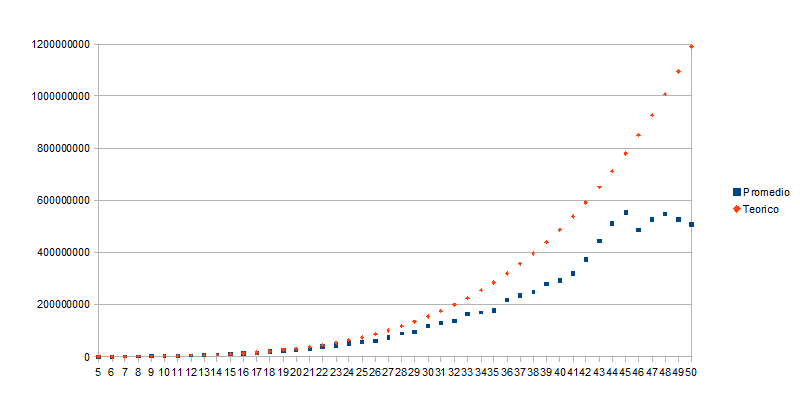
\includegraphics[scale=0.8]{grasp-tiempos-Azar.png}
\caption{Costos}
\end{figure}

\subsubsection{Grafos densos}

\begin{figure}[H]
	\centering
	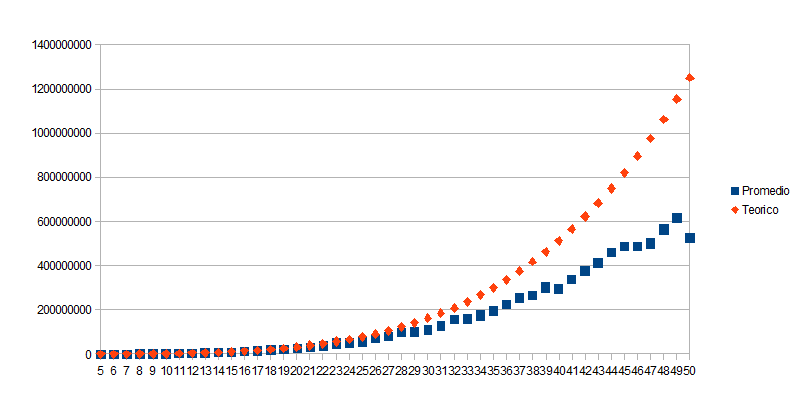
\includegraphics[scale=0.8]{grasp-tiempos-G-y-H-densos.png}
\caption{Costos}
\end{figure}

\subsubsection{G y H complementos}

\begin{figure}[H]
	\centering
	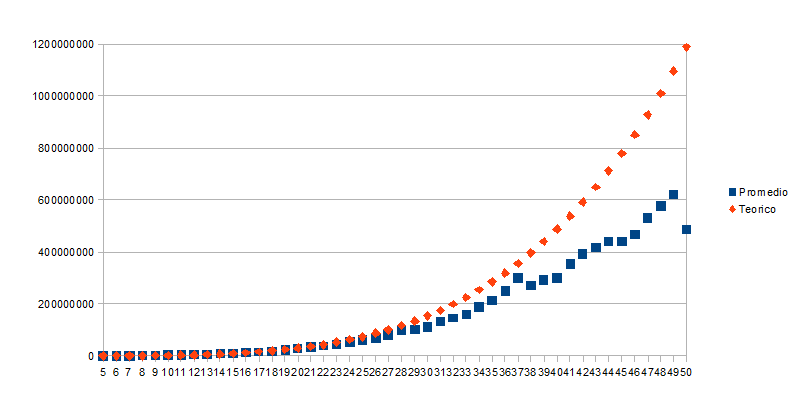
\includegraphics[scale=0.8]{grasp-tiempos-H-complemento.png}
\caption{Costos}
\end{figure}
